\documentclass[../main.tex]{subfiles}
\graphicspath{{\subfix{../img/}}}

\begin{document}

\subsection{Effects of T-Type Channel KD on Minimal Resting Membrane Potential During Bursting}

\noindent An unpublished study by Anatoli Ender, and David Owald reported an increase in the minimal recorded membrane potential following knockdown of the T-type $\text{Ca}^{2+}$ channels (Figure \ref{fig:sleep_r5_knock_ttx_voltage}). The minimal resting membrane potential was defined as the average of the lowest membrane potentials measured during each cycle of the bursting oscillation. This finding may seem counterintuitive, given that the calcium current is depolarizing. Thus, reducing such a current would typically be expected to lower, but not to increase, the membrane potential. The observation suggests the presence of an additional, potentially calcium-dependent, mechanism.

One possible class of mechanisms involves intracellular processes that depend on, or are triggered by calcium.
It has been demonstrated that calcium can activate various signaling cascades in neurons, trigger transcriptional responses in neurons, and affect synaptic scaling \parencite{hagenstonFunctionalConsequencesCalciumDependent2020}. Therefore, a reduction in calcium influx due to T-type channel knockdown could, in principle, influence the synaptic strength between R5 neurons,
or modulate their intrinsic properties (e.g. expression of other ion channels), thereby affecting the minimal resting membrane potential during bursting.

However, another potential mechanism, which does not rely on calcium-dependent changes in intrinsic properties of neurons is the involvement of calcium-activated potassium channels. Since potassium currents are hyperpolarizing, their activation could contribute to setting the minimal resting membrane potential to more hyperpolarized values.
A reduction in calcium influx could potentially lead to a reduced activation of these potassium channels, resulting in the reduced hyperpolarizing current, and, consequently, an increase of the minimal resting membrane potential.

Considering the potential modulation of calcium-dependent synaptic strength, and the contribution of the T-type channels in activating calcium-activated potassium channels, across all implemented models, parameters were set to the values described in Appendix \ref{appendix:functions_and_parameters}, and only the input current and the maximal conductance of the T-type channels were varied. Note that, as discussed in Section \ref{sec:sleep_and_r5_network},
knockdown of the T-type channel could have been incomplete, and what proportion of the channels remaining after the knockdown is unkown. Therefore, the maximal conductance of the T-type channels channels was systematically reduced, rather than set to $0$.

\afterpage{%

    \begin{figure}[!t]
        \centering
        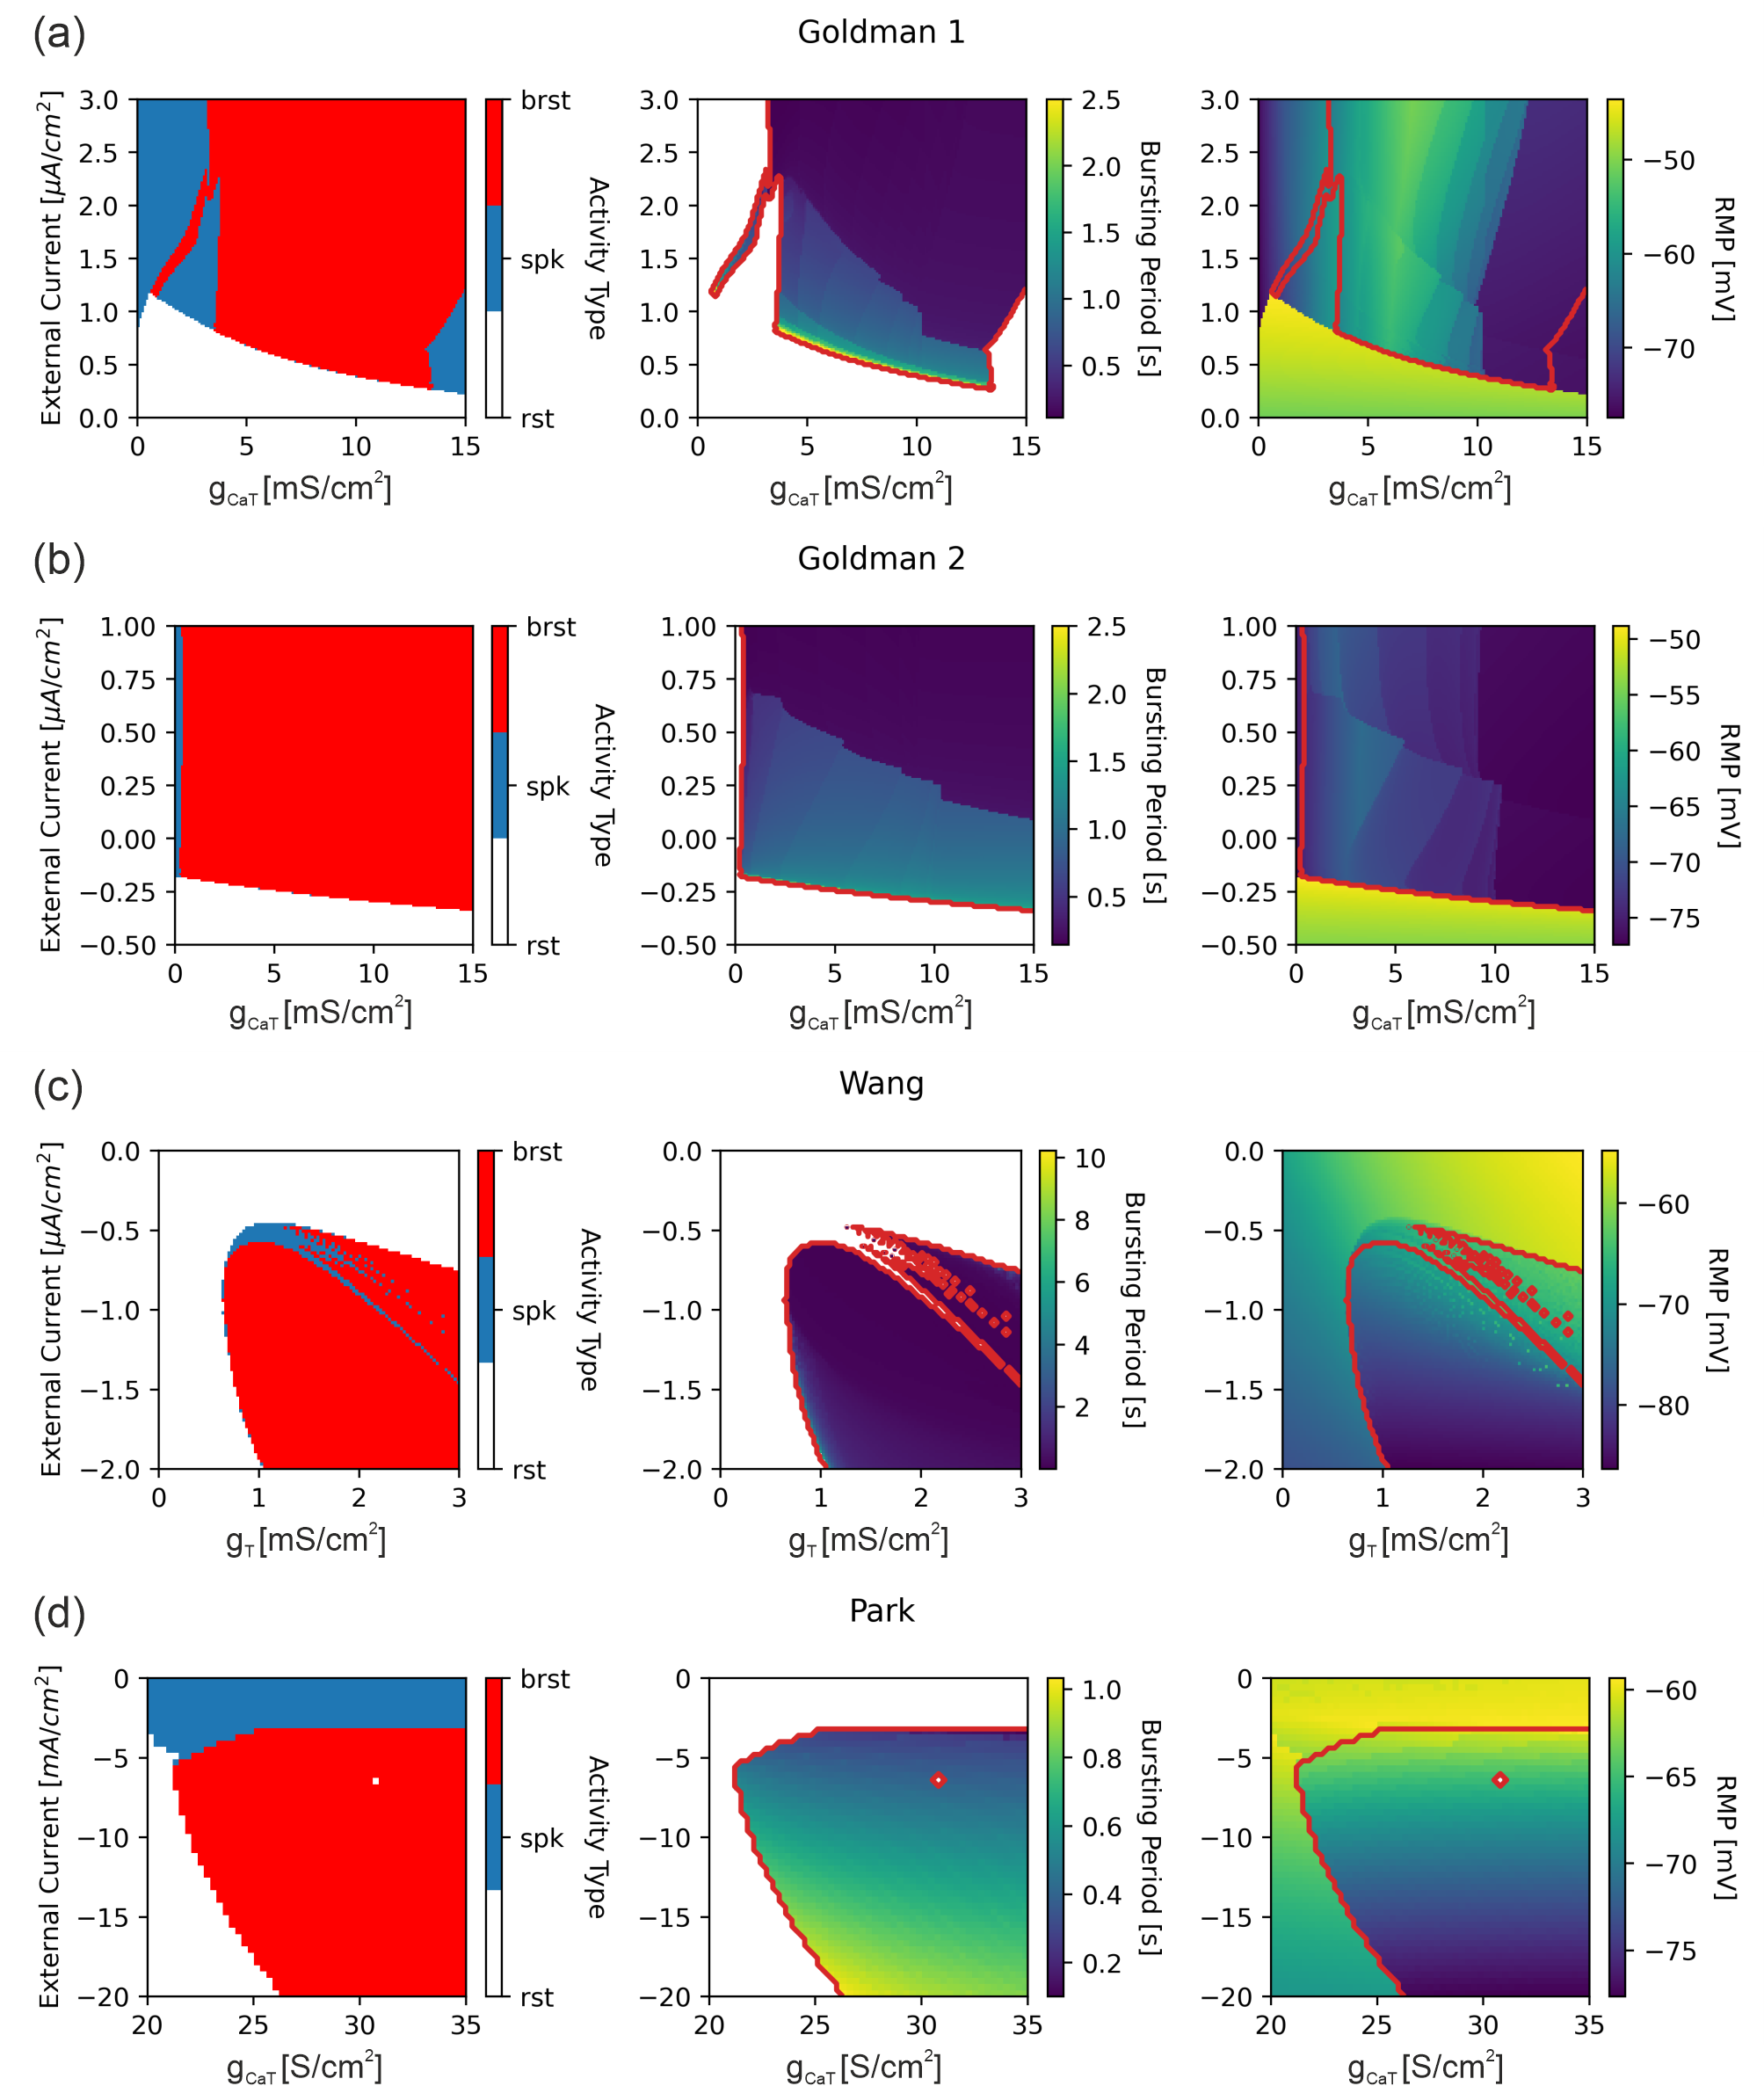
\includegraphics[width=0.95\linewidth]{../img/rmp/rmp_phase.png}
        \caption[Effect of T-type channel conductance and input current on minimal resting membrane potential]{\textbf{Effect of T-type channel conductance and input current on minimal resting membrane potential.} Results for the four implemented models. $x$-axis indicates the maximal conductance of T-type calcium channels, and the $y$-axis shows external input to the neuron. Labels and units match those described in Appendix \ref{appendix:functions_and_parameters}. Left: regions in the I$_\text{ext}$-$g$ parameter plane where models exhibit bursting (red), spiking (blue), or resting (white) activity. Middle: dependence of the bursting period on external input and mT-type channel conductance. Right: dependence of the minimal resting membrane potential on external input and T-type channel conductance. Regions in which the model exhibited bursting are outlined in red.}
        \label{fig:rmp_models_phase}
    \end{figure}

}

Figure \ref{fig:rmp_models_phase}a-d shows the results for the four implemented models (see Section \ref{subsec:results_preface} and Appendix \ref{appendix:functions_and_parameters}).
Note, that the labels on the $x$ axes, as well as the units have been selected to remain consistent with those used in the corresponding papers (see Appendix \ref{appendix:functions_and_parameters}), and both $g_{CaT}$ and $g_T$ refer to the maximal conductance of T-type calcium channels.
The left plots illustrate the regions in the I$_{\text{ext}}$-$g_{CaT}$ parameter plane where each of the investigated models exhibited bursting, spiking, or resting behaviour. The region where the models exhibited bursting behaviour are indicated by a solid red curve in all other plots. The figure also shows the bursting period (middle plots) and the minimal resting membrane potential (right plots) obtained from numerical simulations.

\subsubsection{Modulation of the minimal resting membrane potential by T-type channel knockdown}

Interestingly, a reduction in the maximal conductance of the T-type channels was sufficient to increase the minimal resting membrane potential only in two of the models: Goldman 1 and Goldman 2, as reflected by a shift in color from blue to yellow in the rightmost heatmaps of Figure \ref{fig:rmp_models_phase}. These models are characterized by a relatively high maximal conductance of calcium-activated potassium channels compared to that of the calcium channels (see Figure \ref{fig:model_conductances}).
In contrast, for the other two models, decrease of the maximal T-type conductance was not sufficient to increase the minimal resting membrane potential. Increase of the external current was necessary to induce such an effect.

As mentioned in Section \ref{subsec:results_preface}, the Wang model does not contain calcium-activated potassium channels. In contrast, the Park model includes such channels, however, the corresponding maximal conductance is relatively low in comparison to other conductances (see Figure \ref{fig:model_conductances} and Appendix \ref{appendix:functions_and_parameters}).

The figure illustrates that there are two potential mechanisms by which the experimental observation could be reproduced. The first involves an increase in the external drive to the neuron (Figure \ref{fig:rmp_models_phase}a,d). Since the T-type Ca$^{2+}$ channels were specifically knocked down in R5 neurons, this would imply calcium-dependent postsynaptic changes within R5 neurons that strengthen synaptic connections to the presynaptic cells. However, currently little is known about if, how calcium influences synaptic strength in R5 neurons.

The second mechanism, where the reduction in the maximal T-type channel conductance was sufficient to increase the minimal resting membrane potential suggests the involvement of calcium-activated potassium channels (Figure \ref{fig:rmp_models_phase}b,c).

Given that this thesis focuses on the role of calcium-activated potassium channels in modulating the minimal resting membrane potential, in the following, the analysis will focus on the two models in which a reduction in the maximal conductance of T-type channels resulted in increased minimal resting membrane potential - namely the Goldman 1 and Goldman 2 models.

\afterpage{%
\begin{figure}[!t]
    \centering
    \textbf{Goldman 1 Model} \\[1ex]  % Title at top center
    % First row
    \begin{subfigure}[t]{0.48\textwidth}
        \centering
        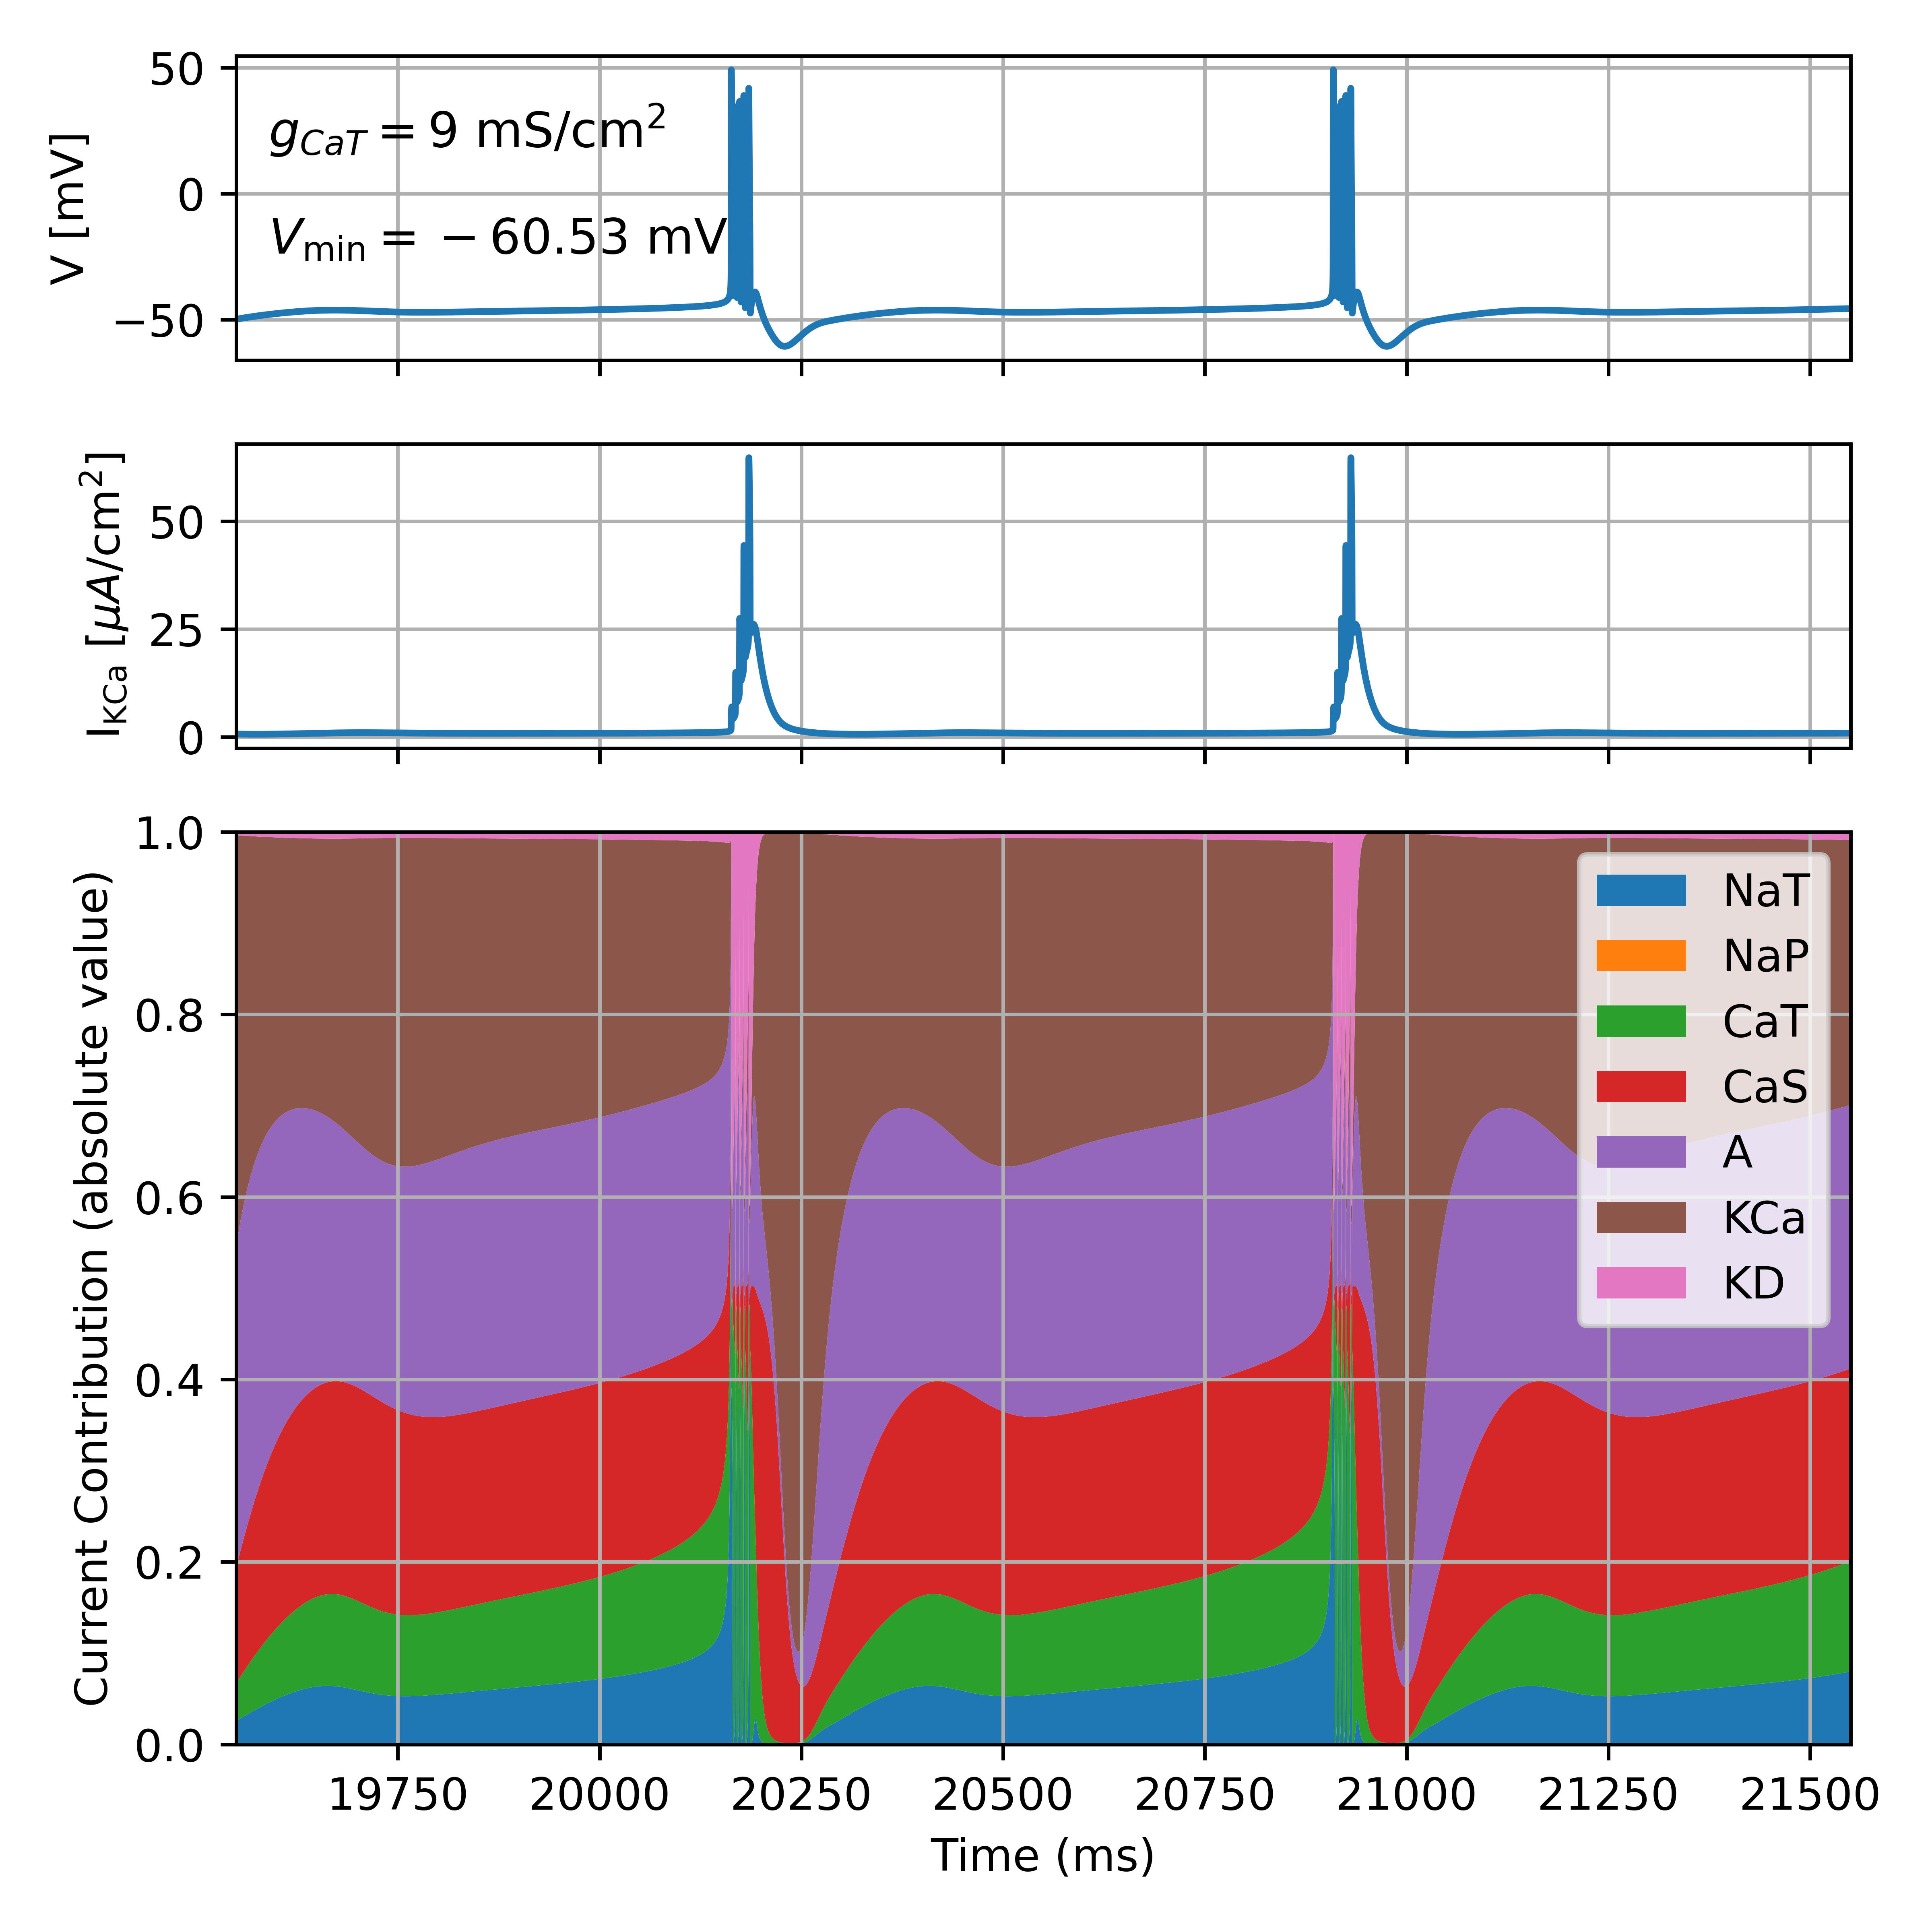
\includegraphics[width=\linewidth]{../img/rmp/goldman_1_g_9.png}
        \label{fig:rmp_models_contrib_10_goldman_1}
    \end{subfigure}
    \hfill
    \begin{subfigure}[t]{0.48\textwidth}
        \centering
        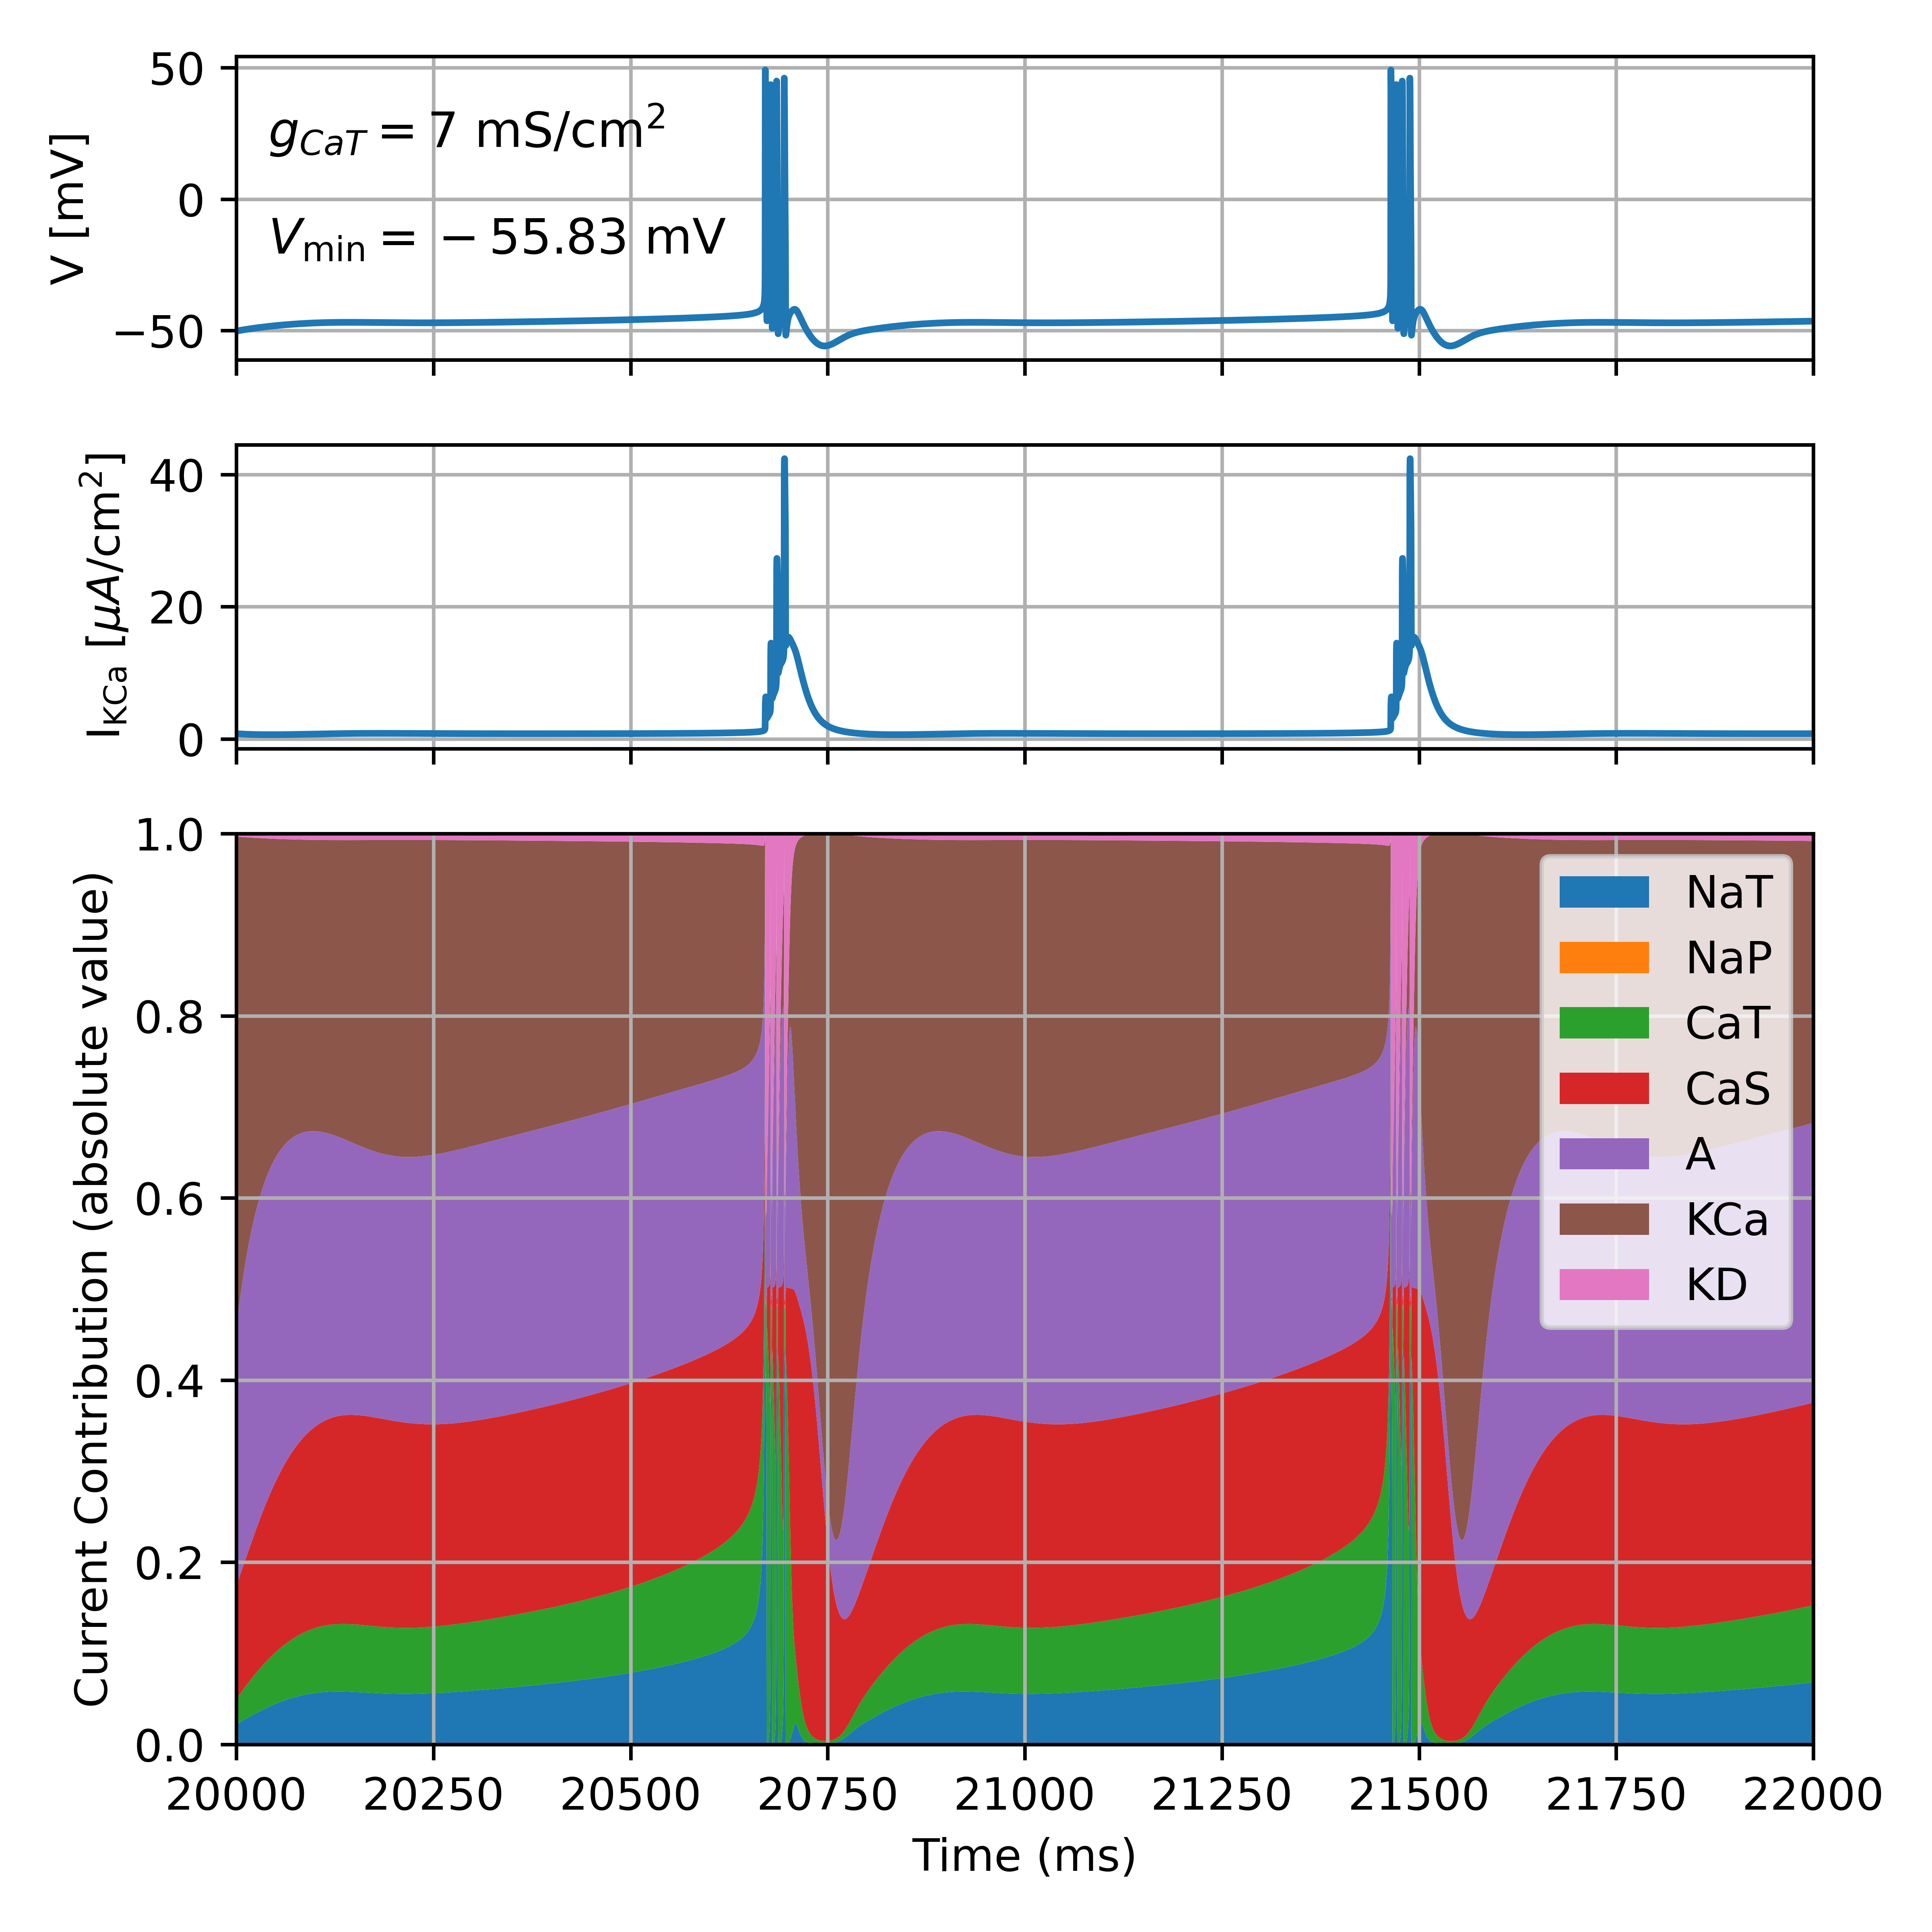
\includegraphics[width=\linewidth]{../img/rmp/goldman_1_g_7.png}
        \label{fig:rmp_models_contrib_5_goldman_1}
    \end{subfigure}

    \textbf{Goldman 2 Model} \\[1ex]  % Title at top center

    % First row
    \begin{subfigure}[t]{0.48\textwidth}
        \centering
        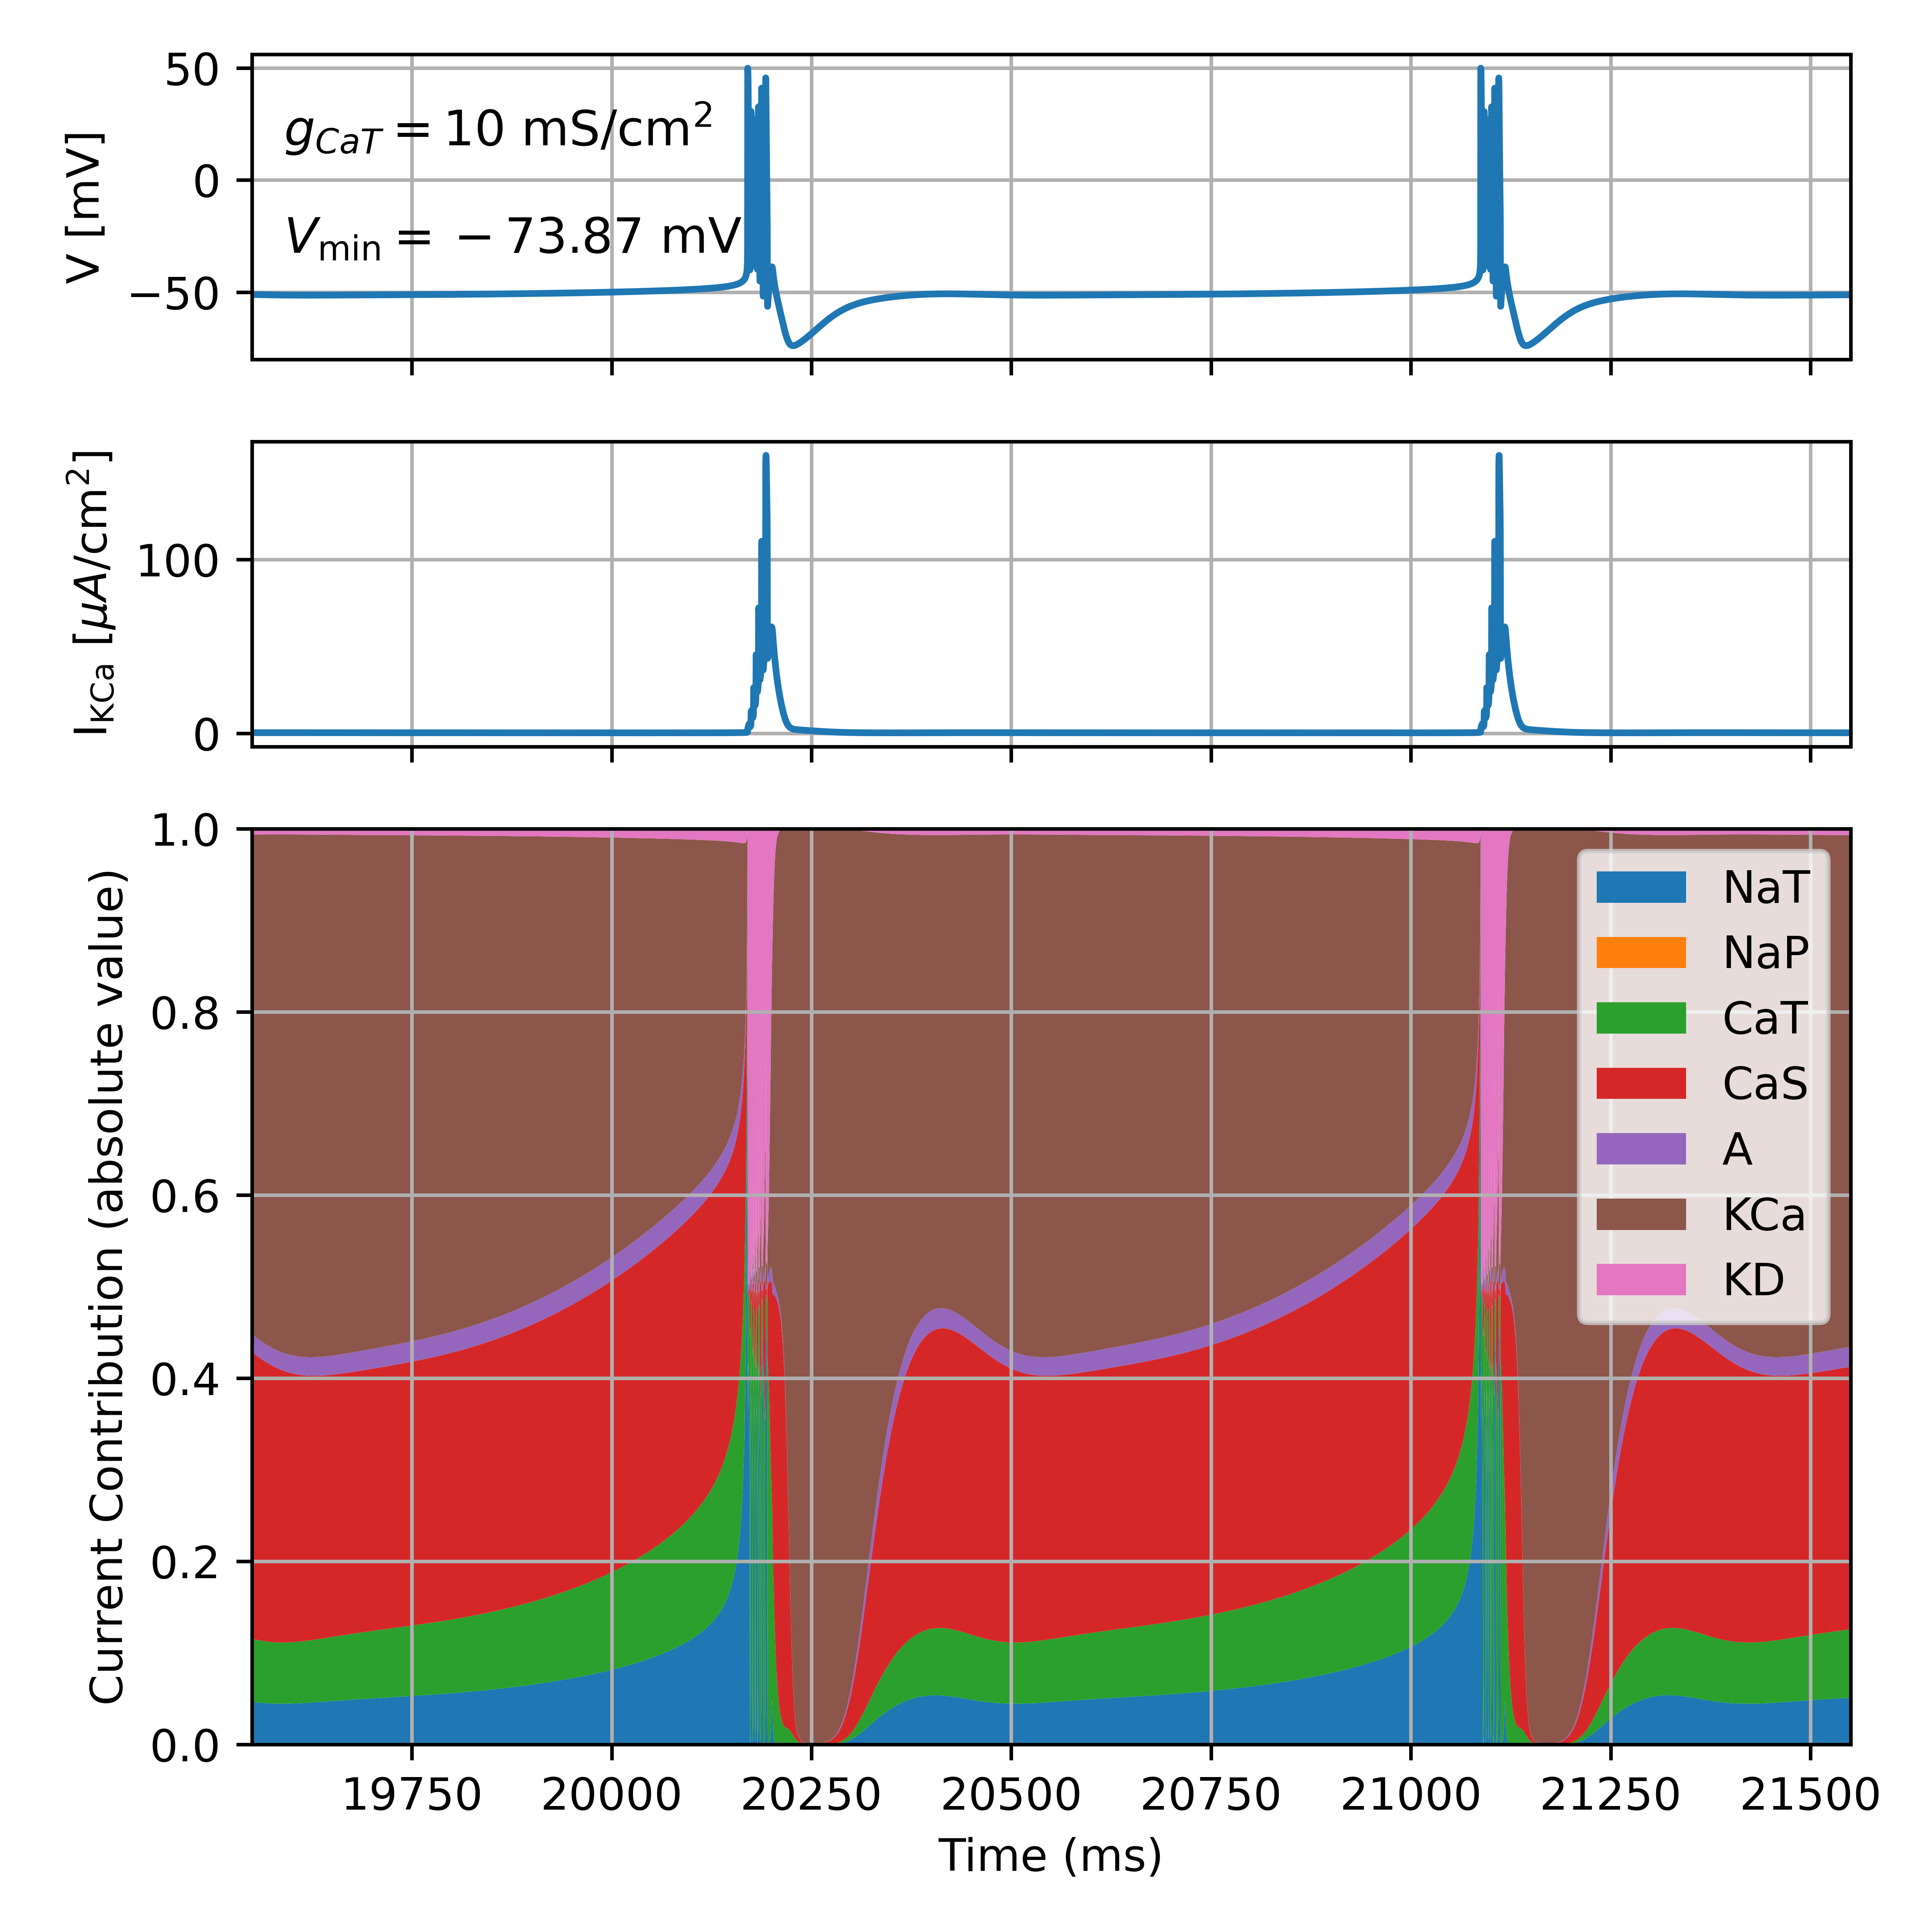
\includegraphics[width=\linewidth]{../img/rmp/goldman_2_g_10.png}
        \label{fig:rmp_models_contrib_10_goldman_2}
    \end{subfigure}
    \hfill
    \begin{subfigure}[t]{0.48\textwidth}
        \centering
        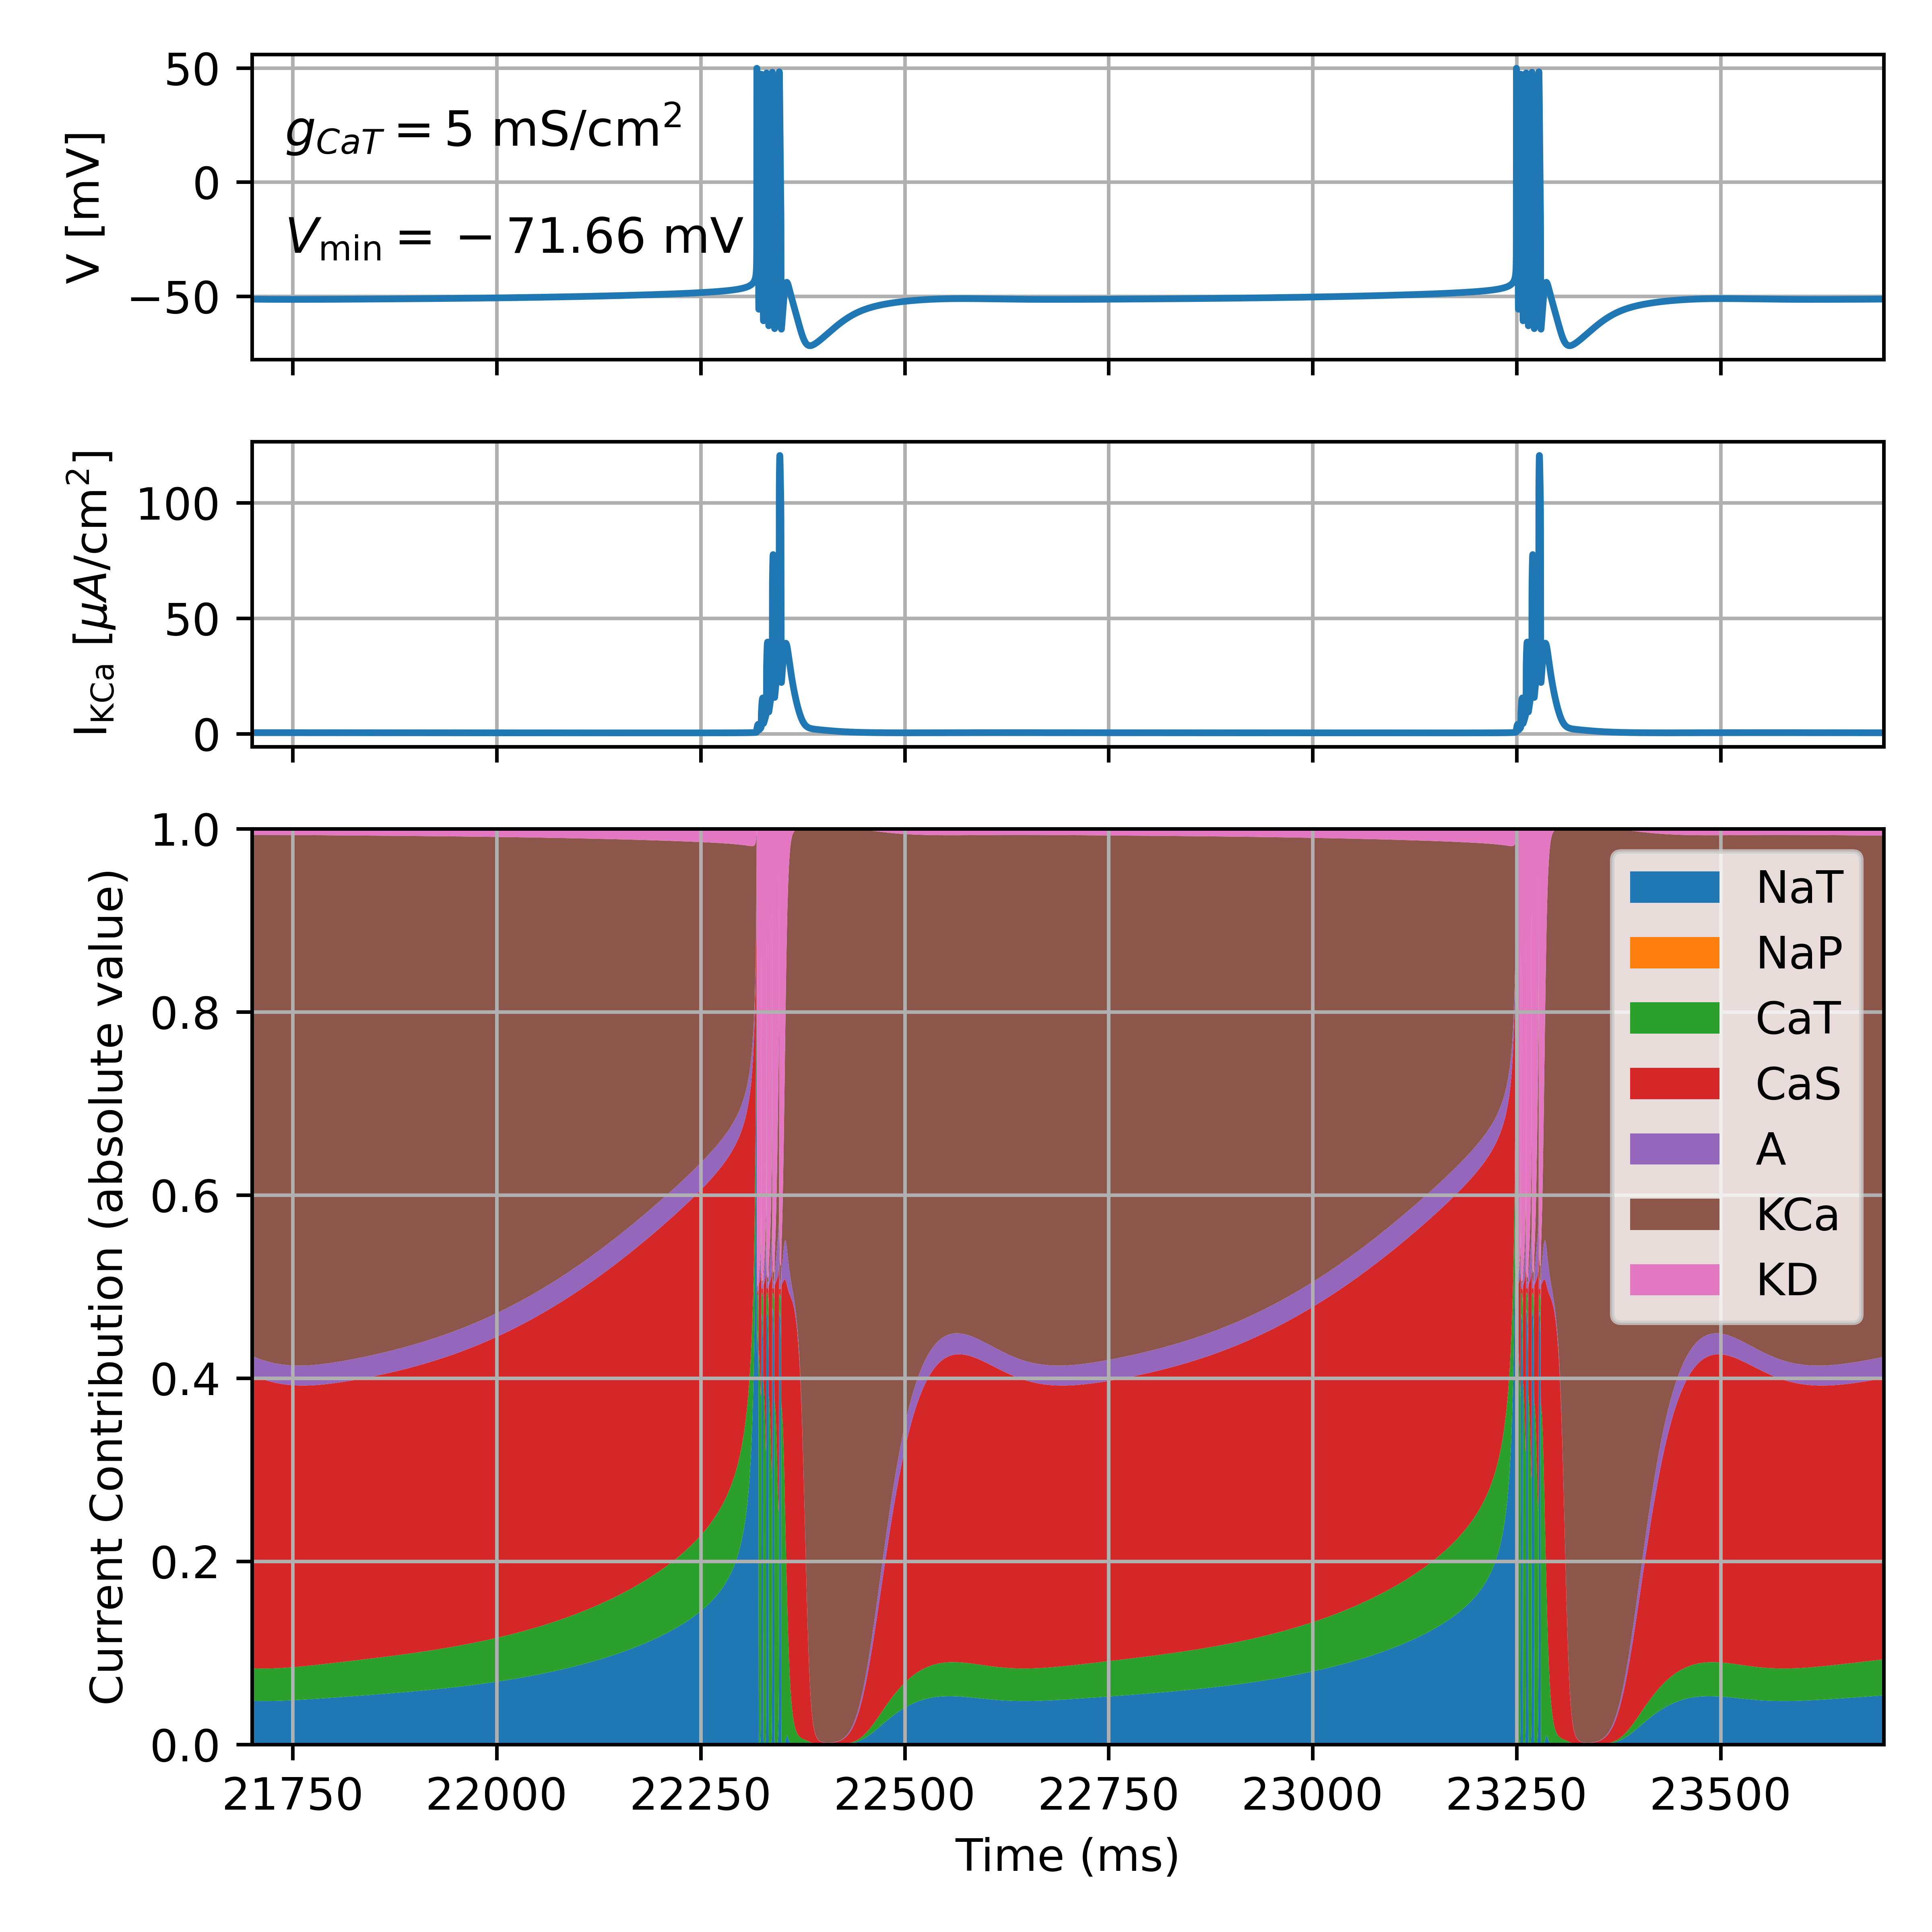
\includegraphics[width=\linewidth]{../img/rmp/goldman_2_g_5.png}
        \label{fig:rmp_models_contrib_5_goldman_2}
    \end{subfigure}
    
    \caption[Contribution of the calcium-activated potassium channel on the minimal resting membrane potential]{\textbf{Contribution of calcium-activated potassium channel on minimal resting membrane potential.} Results shown for the Goldman 1 and Goldman 2 models, with the external input current set to $1$ $\mu S/\text{cm}^2$ for Goldman 1, and to $0$ for the Goldman 2 model. Parameter values for the maximal conductance of the T-type channels are indicated as text in each figure. All other parameters were held constant, as described in Appendix \ref{appendix:functions_and_parameters}. Top: voltage trace, with the corresponding minimal resting membrane potential indicated as text. Middle: current through the calcium-activated potassium channel (KCa). Bottom: stack plot showing the relative contribution of each ionic current at each simulation time step (see main text for details).}
    \label{fig:rmp_models_contrib_fig_goldman}
\end{figure}
}

% Several observations can be made from the figure. First, the modulation of the minimal resting membrane potential by the maximal conductance of the T-type calcium channels is more pronounced in the Goldman 1 model in comparison to the Goldman 2 model (\textcolor{red}{Increase gKCa (25-40), increase in CaT (7-10), decrease in CaS 10.5 - 8}). Second, there are regions where the minimal resting membrane potential changes abruptly with variations in T-type conductance. Third, when decreasing the maximal conductance of the T-type channel, the minimal resting membrane potential decreases, rather than increases, near the transition from bursting to spiking (comare the regions outlined by the red curve to the area in the left plot where the model transitions from bursting (red) to spiking (blue); this effect is illustrated more clearly in Figure \ref{fig:rmp_models_phase_i_slices}). These aspects will be further discussed in the remainder of this section.


\subsubsection{Contribution of Ca$^{2+}$-activated K$^+$ channels to the minimal resting membrane potential}

\noindent To investigate whether calcium-activated potassium channels are responsible for the change in the minimal resting membrane potential observed in Figure \ref{fig:rmp_models_phase}a-b, the relative contribution of each current was analyzed in representative simulations in which the model exhibited approximately $1$ Hz bursting.

The contribution of each current was defined as the percentage of its magnitude relative to the sum of the absolute values of all ionic currents. The results are shown in Figure \ref{fig:rmp_models_contrib_fig_goldman} for the Goldman 1 and Goldman 2 models, along with the corresponding voltage trace and the current through the calcium-activated potassium channel (KCa). In the stack plots, the height of each colored region represents the percentage of the magnitude of that current relative to the total ionic current at each time point of the simulation.

In Figure \ref{fig:rmp_models_contrib_fig_goldman}, the relative contribution of the calcium-activated potassium channels are indicated by the brown area. Comparing the height of this region to the voltage trace (top plots), one can observe that the minimal resting membrane is larely mediated by these channels (Goldman 1: $77.53\%$ for $g_{CaT}=7$ mS/cm$^2$ and $89.82\%$ for $g_{CaT}=9$ mS/cm$^2$; Goldman 2: $99.92\%$ for $g_{CaT}=10$ mS/cm$^2$ and $99.82\%$ for $g_{CaT}=5$ mS/cm$^2$). Note that the stackplot at the bottom illustrates the relative contributions of the currents. Although the KCa current is strongest during spikes, its relative contribution is greater than that of other currents at the minimal resting membrane potential.

Interestingly, although the minimal resting membrane potential was more strongly mediated by calcium-activated potassium channels in the Goldman 2 model, Figure \ref{fig:rmp_models_phase}b-c shows that the modulation of the minimal resting membrane potential is more pronounced in the Goldman 1 model, as indicated by the colors in the heatmaps. Furthermore, as illustrated in Figure \ref{fig:rmp_models_contrib_fig_goldman}, the contribution of the KCa channel is more robust to changes in T-type conductance in the Goldman 2 model. Specifically, reducing the conductance from $10$ mS/cm$^2$ to $5$ mS/cm$^2$ in the Goldman 2 model has a smaller effect on the KCa contribution than reducing it from $9$ mS/cm$^2$ to $7$ mS/cm$^2$ in the Goldman 1 model.

The Goldman 1 and Goldman 2 models differ only by the maximal conductances of the ion channels (see Appendix \ref{appendix:functions_and_parameters}, and Figure \ref{fig:model_conductances}). Apart from differences in other conductances, the maximal conductance of the calcium activated potassium channel is lower in Goldman 1 in comparison to Goldman 2 models (Goldman 1: $g_{CaT}=7$ mS/cm$^2$, $g_{KCa}=25$ mS/cm$^2$; Goldman 2: $g_{CaT}=10$ mS/cm$^2$, $g_{KCa}=40$ mS/cm$^2$). Even a small influx of calcium could potentially result in domination of the KCa-mediated currents if the maximal conductance of the KCa channels is large enough.

\color{red}

To test this - vary g\_CaT + g\_KCa and: (Todo) 1. (!IMPORTANT!) Plot similar figures as in Figure \ref{fig:rmp_models_phase}, but with colour showing total calcium influx during burst, total t-type current during burst, total t-type current during burst, total calcium current during burst, total KCa current after burst before plateau.
BUT: x axis - CaT channel and y axis KCa to see how the calcium AND KCa conductance affects resting membrane potential

\color{black}


\subsubsection{Non-monotonic trends and abrupt shifts in activity}

Figure \ref{fig:rmp_models_phase_i_slices} shows the values of the minimal resting membrane potentials from Figure \ref{fig:rmp_models_phase}, plotted against $g_{CaT}$ for fixed values of the external current. The figure illustrates that in certain regions of the I$_{\text{ext}}$-$g_{CaT}$ parameter space, decreasing the maximal conductance of the T-type channels leads to a decrease in the minimal membrane potetial contrary to the behaviour observed for larger values of $g_{CaT}$ (see the curve right to the shaded area in Figure \ref{fig:rmp_models_phase_i_slices}).

To better understand this behaviour, representative voltage traces were examined around the critical point where the minimal resting membrane potential begins to decrease as $g_{CaT}$ is reduced (Figure \ref{fig:rmp_models_phase_i_slices_voltage}) \textcolor{red}{(Describe plot, where?)}. The figure shows that this drop in minimal potential likely corresponds to the presence of spike undershoots that fall below the membrane potential at rest (i.e. potential where the model neurons do not exhibit spikes).

% Since in R5 neurons the observed membrane potential during bursts is strictly greater than during the interburst interval (Figure \ref{fig:sleep_r5_knock_ttx_voltage}), could the above-described result indicate a partial blockade of the T-type channels? \textcolor{red}{(What should one concentrate on?)}
% Not necessarily. As illustrated in Sections \ref{sec:sleep_and_r5_network} and \ref{sec:math_background}, even within the low-dimensional fast-slow system framework, bursting can arise through various mechanisms, depending on the nature of burst onset and offset. Moreover, variation in the maximal conductances of single channels has been shown to produce qualitatively different effects, even within the same model, when operating in different parameter regimes - despite exhibiting similar voltage traces under default parameters (i.e. before the variation in single conductances) \parencite{alonsoVisualizationCurrentsNeural2019}. Thus, this effect \textcolor{red}{(which effect?)} is likely model-specific rather than general. Since this region \textcolor{red}{(what region?)} does not appear to be relevant in understanding the electrophysiological properties of the R5 neurons, it was not analyzed further.


\begin{figure}[!t]
    \centering
    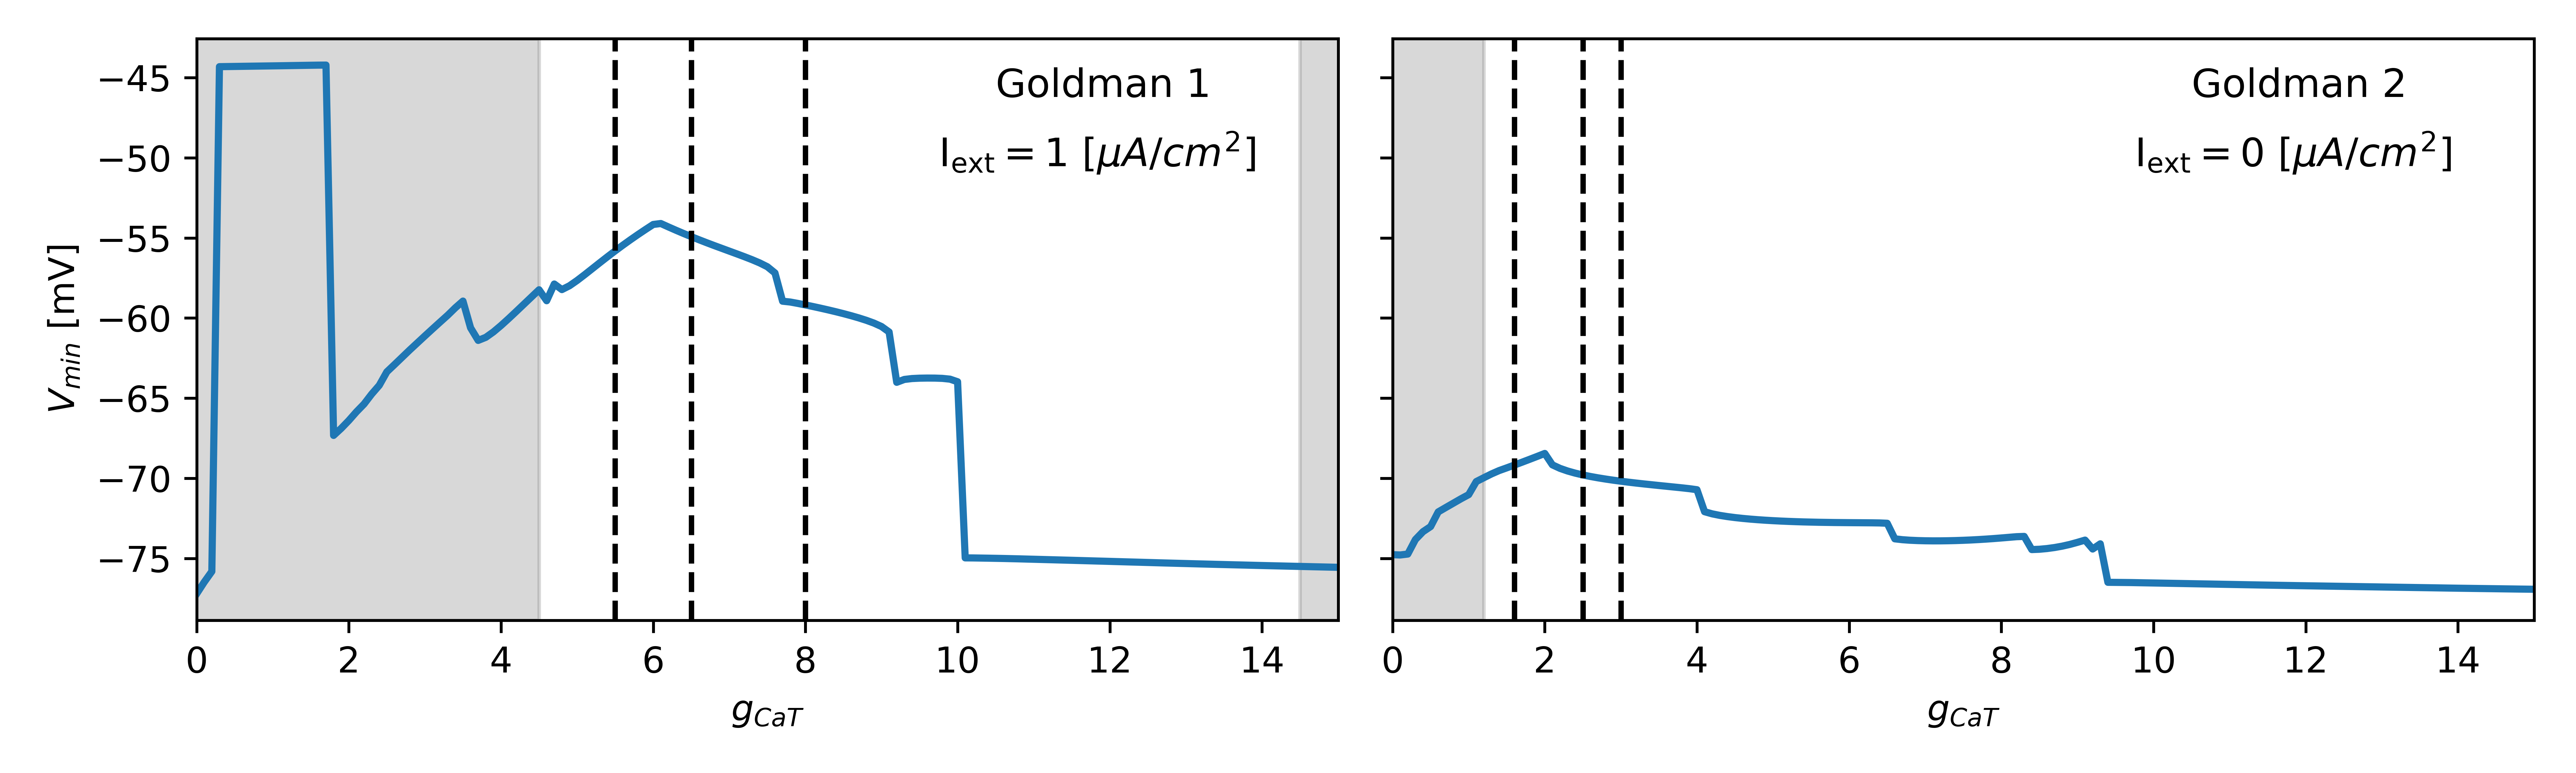
\includegraphics[width=0.9\linewidth]{../img/rmp/goldman_1_2_i_slices.png}
    \caption[Dependence of minimal resting membrane potential on T-type conductance]{\textbf{Dependence of minimal resting membrane potential on T-type conductance.} The figure shows the values of the minimal resting membrane potential along a horizontal slice of the corresponding heatmap shown in Figure \ref{fig:rmp_models_phase}ab for the Goldman 1 (left) and Goldman 2 (right) models. The corresponding values of the external current are indicated by the text within each plot. Grey areas represent regions where the models did not exhibit bursting behaviour. Vertical dashed lines indicate the parameter values for the T-type conductance for which the simulated membrane potential traces are shown in Figure \ref{fig:rmp_models_phase_i_slices_voltage}.}
    \label{fig:rmp_models_phase_i_slices}
\end{figure}

\begin{figure}[!t]
    \centering
    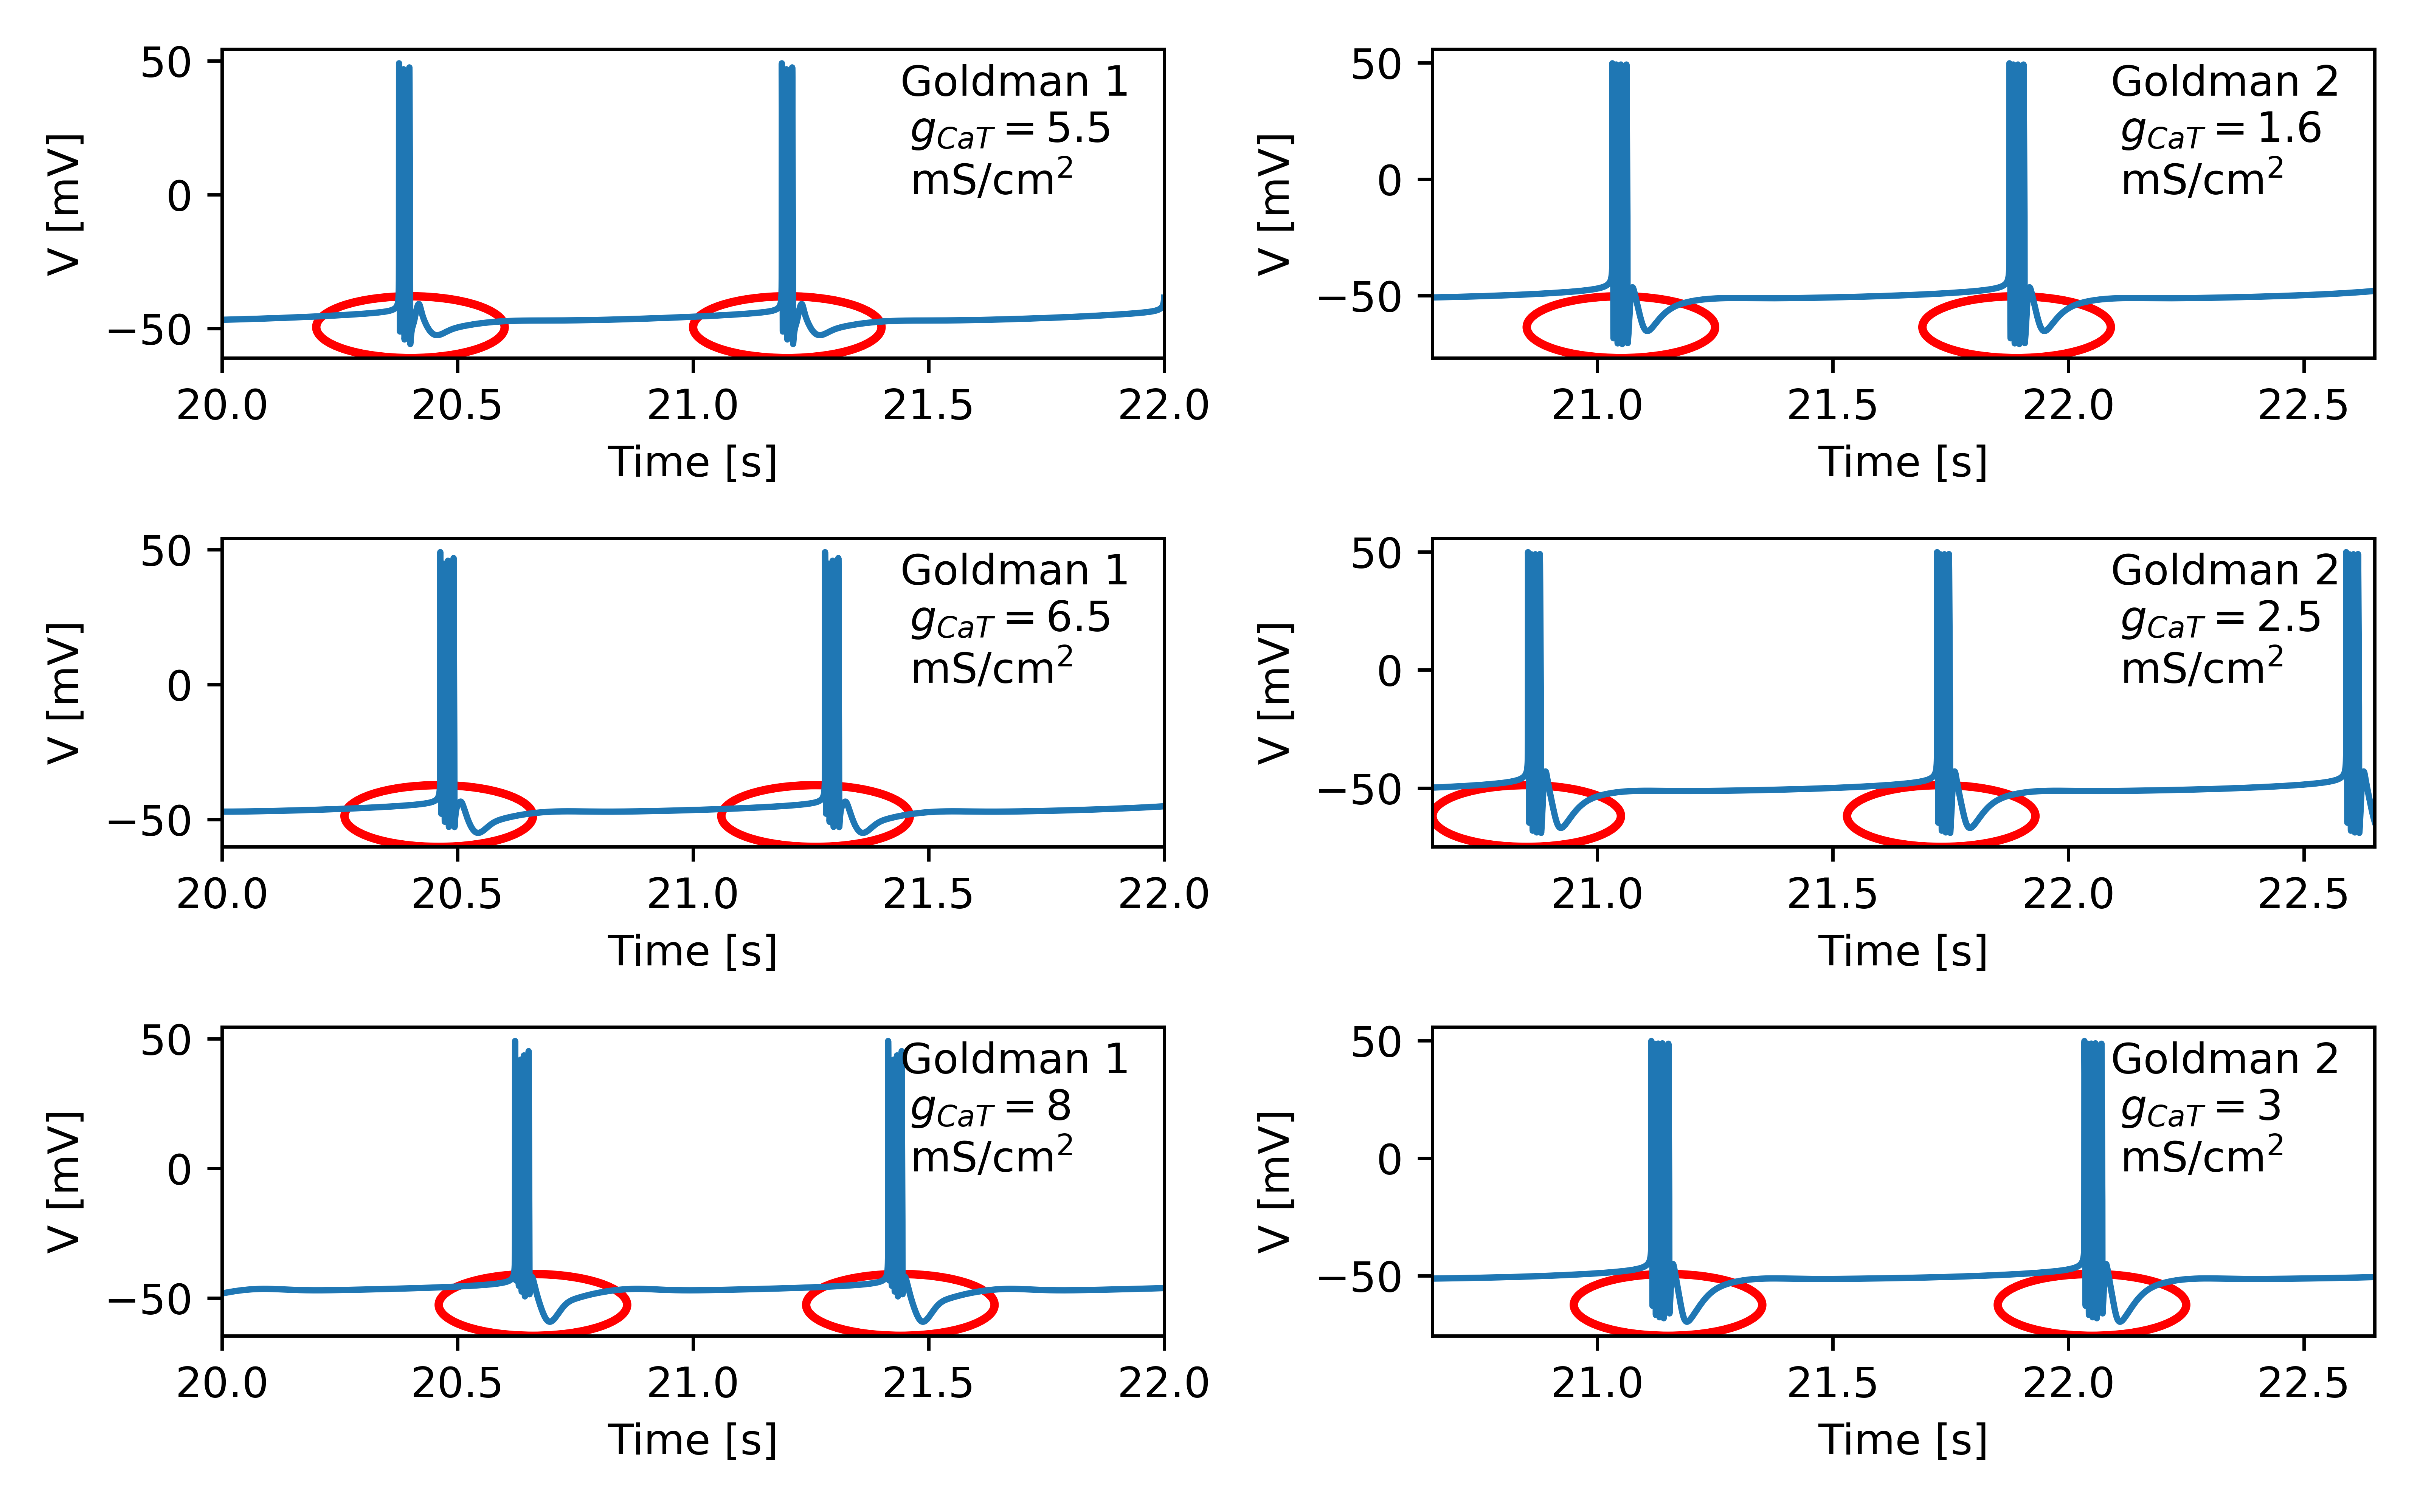
\includegraphics[width=\linewidth]{../img/rmp/goldman_1_2_i_slices_vtraces.png}
    \caption[Voltage traces across the turning point in minimal resting membrane potential]{\textbf{Voltage traces across the turning point in minimal resting membrane potential.} The figure shows representative voltage traces of the model neurons for parameter values corresponding to the dashed lines in Figure \ref{fig:rmp_models_phase_i_slices}. For both models, decreasing the maximal conductance of T-type channels results in an undershoot of the spikes below the membrane potential at rest (i.e. when the model neuron exhibits no spikes).}
    \label{fig:rmp_models_phase_i_slices_voltage}
\end{figure}

\vspace*{3mm}

A narrow region in the $I_{\text{ext}}$-$g_{CaT}$ parameter space of the Goldman 1 model shows a transition from bursting to spiking with small changes in either of the two parameters.
This region appears as a thin red strip in Figure \ref{fig:rmp_models_phase}b left, located between the blue (spiking) areas in the left plot.

Figure \ref{fig:nonlinearity_rmp} shows the same plot as \ref{fig:rmp_models_phase}b on the left, with the voltage traces of the simulations corresponding to the parameter values indicated by the 'x' markers on the heatmap. For $g_{\text{CaT}}=2.3$ mS/cm$^2$ and $I_{\text{ext}}=1.2$ $\mu$A/cm$^2$ the model exhibits spiking behaviour (Figure \ref{fig:nonlinearity_rmp} top right). With increasing external current the system undergoes period-doubling bifurcation (Figure \ref{fig:nonlinearity_rmp} middle right). With further increased external current the system exhibits high-frequency spiking (Figure \ref{fig:nonlinearity_rmp} top right).

\color{red}



2. If have time after finishing everything else: add "non-biologically plausible" calcium current to wang: steap activation time constant as for EAG, but with longer time constant to see the effect there. The result will not change much, maybe one more sentence in the discussion.

\color{black}

\begin{figure}[!t]
    \centering
    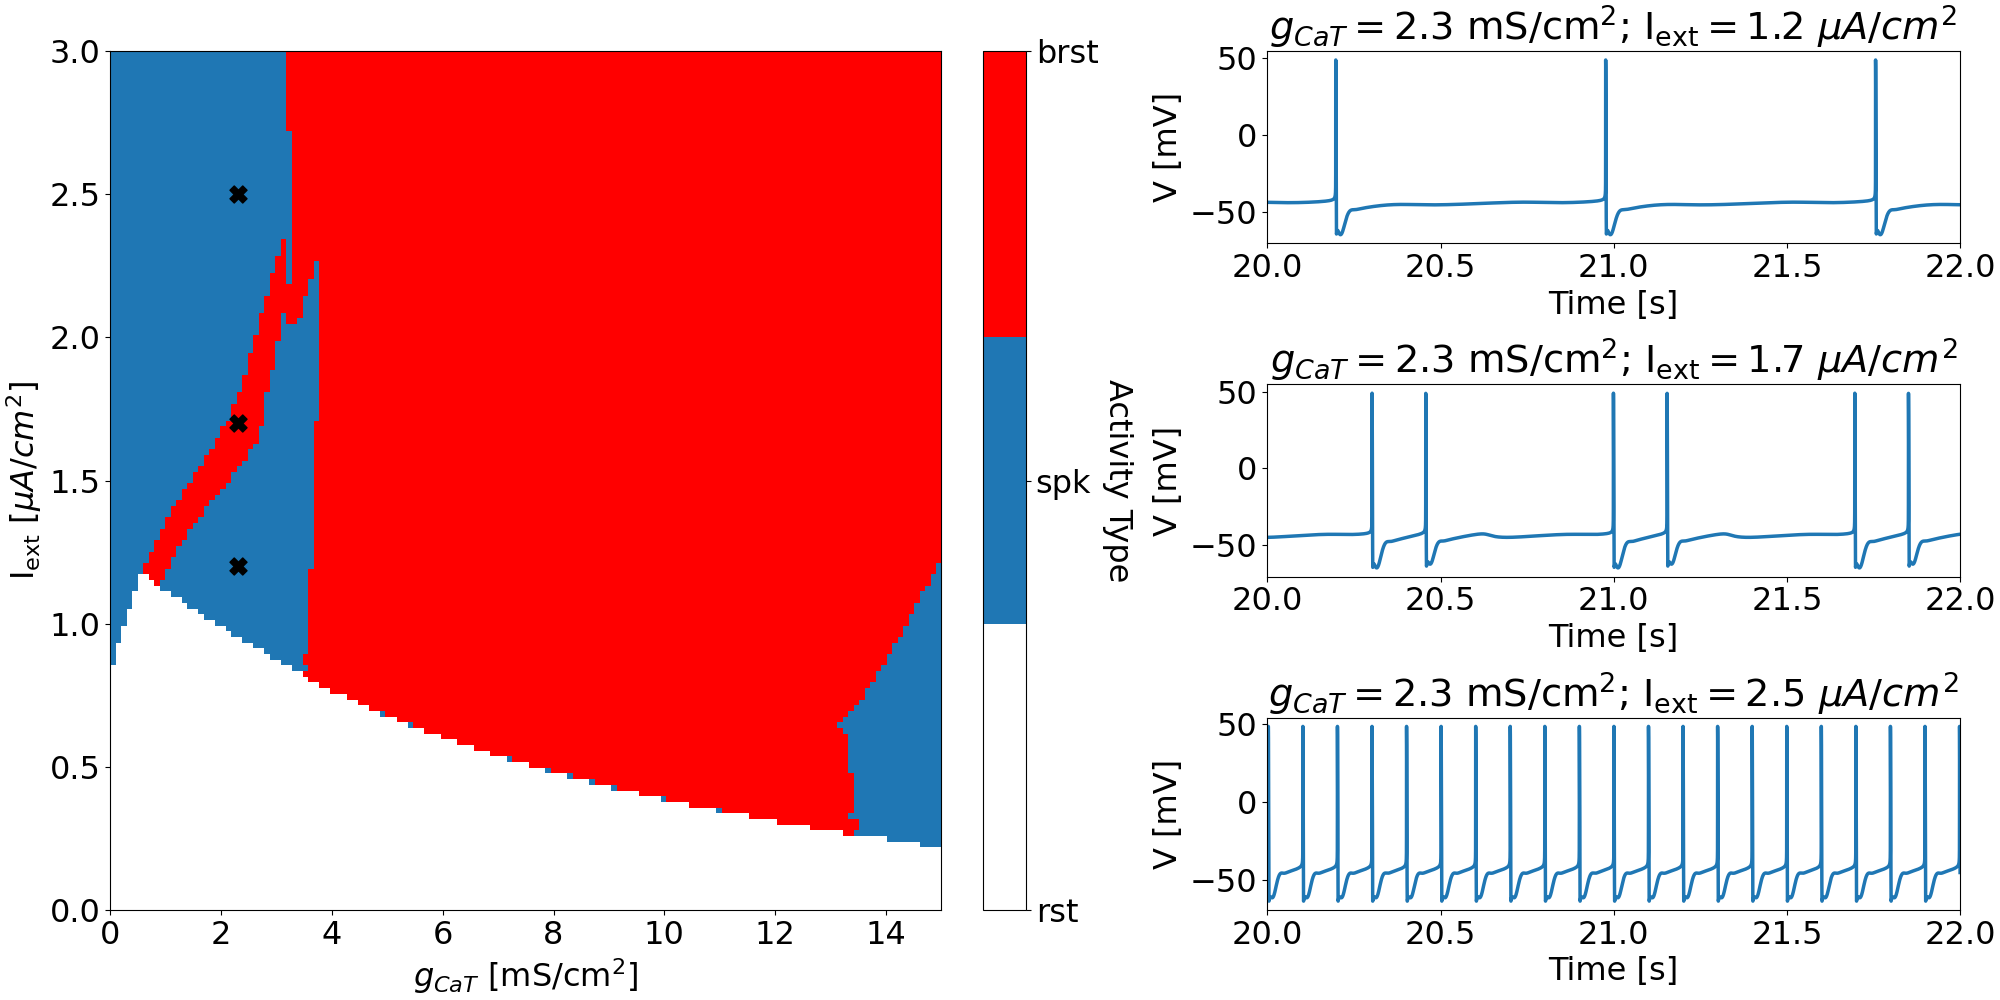
\includegraphics[width=\linewidth]{../img/rmp/nonlinearity_rmp.png}
    \caption[Assessment of the nonlinear region in the Goldman 1 model within the I$_{\text{ext}}$-$g_{\text{CaT}}$ parameter space]{
        \textbf{Assessment of the nonlinear region in the Goldman 1 model within the I$_{\text{ext}}$-$g_{\text{CaT}}$ parameter space.} Left: Minimal resting membrane potential plotted against the external input current (I$_{\text{ext}}$) and the maximal conductance of the T-type channel ($g_{\text{CaT}}$) for the Goldman 1 model (same as in Figure \ref{fig:rmp_models_phase}b left). Right:  Representative voltage traces obtained from simulations using the values of I$_{\text{ext}}$ and $g_{\text{CaT}}$ indicated by the red 'x' markers on the heatmap. All other parameters were set as described in Appendix \ref{appendix:functions_and_parameters}. The narrow region in parameter space indicated by the narrow red "strip" indicates to the period-doubling bifurcation.
    }
    \label{fig:nonlinearity_rmp}
\end{figure}
    


\end{document}